\chapter{Boxplots}

In this chapter, we will work towards creating the boxplot below. We
will take you from a basic boxplot and explain all the customisations we
add to the code step-by-step.

\begin{center}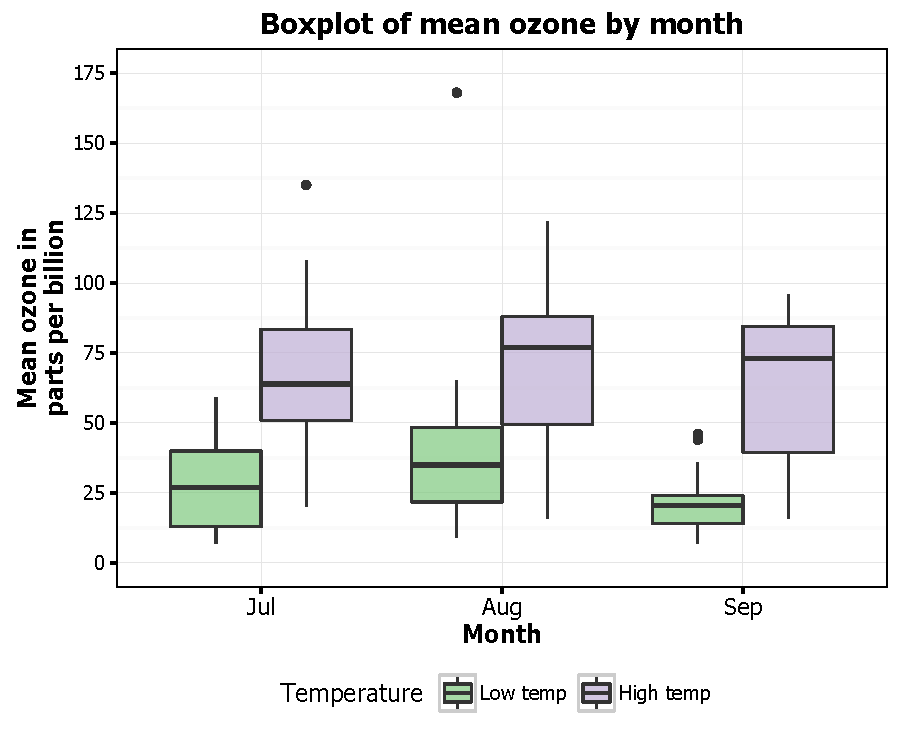
\includegraphics[width=0.6\linewidth]{10_Boxplots_pdf/box_final-1} \end{center}

The first thing to do is load in the data and the libraries, as below.
We'll convert \texttt{Month} into a labelled factor in order to use it
as our grouping variable.

\begin{Shaded}
\begin{Highlighting}[]
\KeywordTok{library}\NormalTok{(datasets)}
\KeywordTok{library}\NormalTok{(ggplot2)}
\KeywordTok{library}\NormalTok{(ggthemes)}
\KeywordTok{library}\NormalTok{(grid)}
\KeywordTok{library}\NormalTok{(RColorBrewer)}

\KeywordTok{data}\NormalTok{(airquality)}
\NormalTok{airquality$Month <-}\StringTok{ }\KeywordTok{factor}\NormalTok{(airquality$Month, }
    \DataTypeTok{labels =} \KeywordTok{c}\NormalTok{(}\StringTok{"May"}\NormalTok{, }\StringTok{"Jun"}\NormalTok{, }\StringTok{"Jul"}\NormalTok{, }\StringTok{"Aug"}\NormalTok{, }\StringTok{"Sep"}\NormalTok{))}
\end{Highlighting}
\end{Shaded}

\section{Basic boxplot}\label{basic-boxplot}

In order to initialise a plot we tell ggplot that \texttt{airquality} is
our data, and specify that our x-axis plots the \texttt{Month} variable
and our y-axis plots the \texttt{Ozone} variable. We then instruct
ggplot to render this as a boxplot by adding the
\texttt{geom\_boxplot()} option.

\begin{Shaded}
\begin{Highlighting}[]
\NormalTok{p10 <-}\StringTok{ }\KeywordTok{ggplot}\NormalTok{(airquality, }\KeywordTok{aes}\NormalTok{(}\DataTypeTok{x =} \NormalTok{Month, }\DataTypeTok{y =} \NormalTok{Ozone)) +}\StringTok{ }
\StringTok{  }\KeywordTok{geom_boxplot}\NormalTok{()}
\NormalTok{p10}
\end{Highlighting}
\end{Shaded}

\begin{center}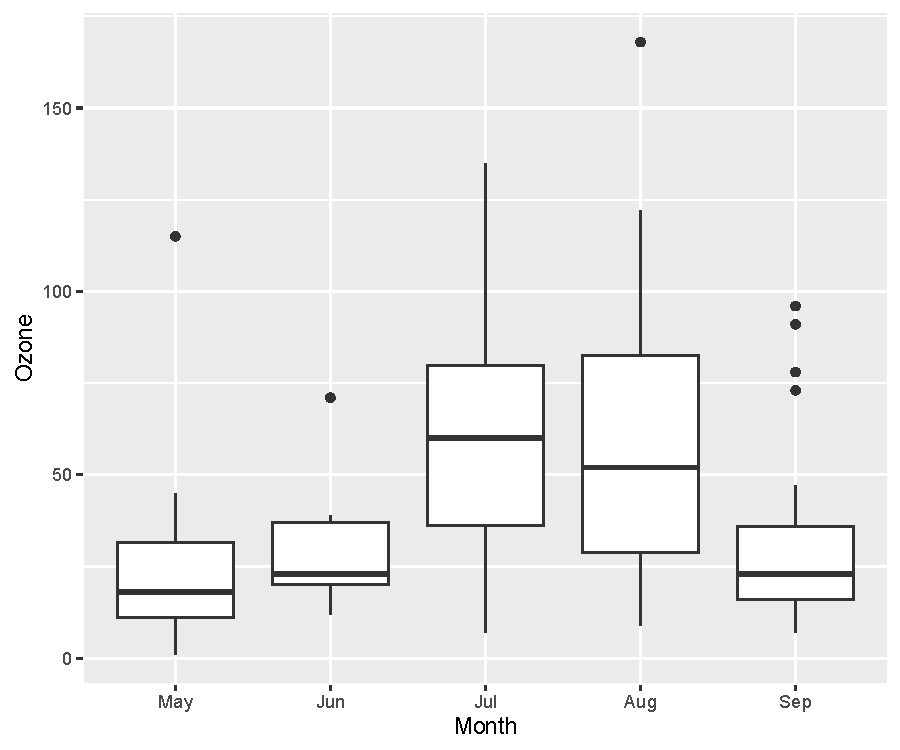
\includegraphics[width=0.6\linewidth]{10_Boxplots_pdf/box_1-1} \end{center}

\section{Customising axis labels}\label{customising-axis-labels}

In order to change the axis labels, we have a couple of options. In this
case, we have used the \texttt{scale\_x\_discrete} and
\texttt{scale\_y\_continuous} options, as these have further
customisation options for the axes we will use below. In each, we add
the desired name to the \texttt{name} argument as a string.

\begin{Shaded}
\begin{Highlighting}[]
\NormalTok{p10 <-}\StringTok{ }\NormalTok{p10 +}\StringTok{ }\KeywordTok{scale_x_discrete}\NormalTok{(}\DataTypeTok{name =} \StringTok{"Month"}\NormalTok{) +}
\StringTok{  }\KeywordTok{scale_y_continuous}\NormalTok{(}\DataTypeTok{name =} \StringTok{"Mean ozone in parts per billion"}\NormalTok{)}
\NormalTok{p10}
\end{Highlighting}
\end{Shaded}

\begin{center}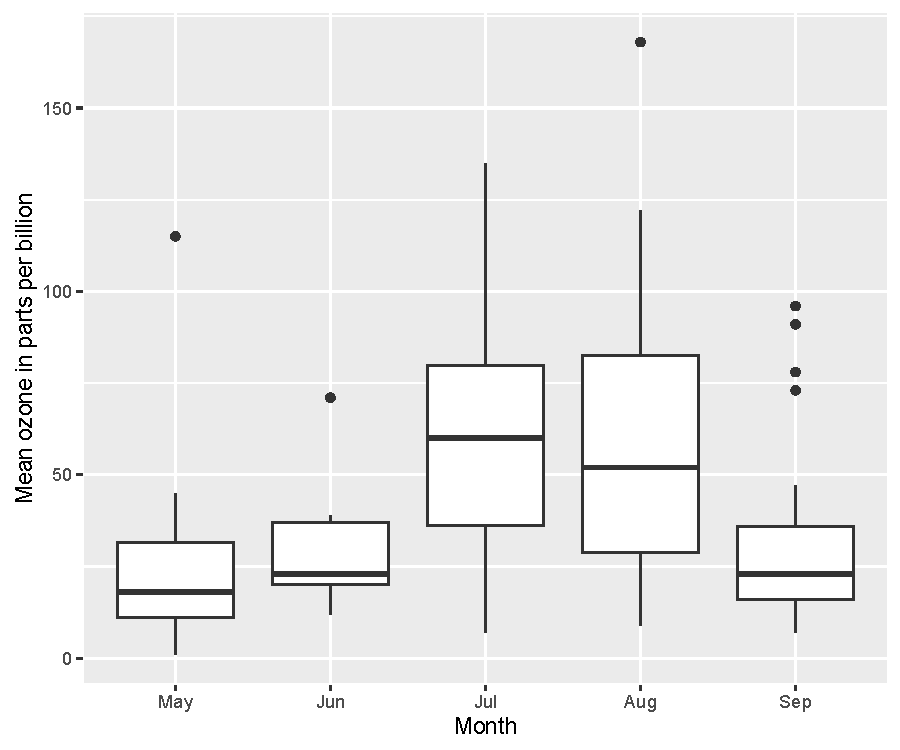
\includegraphics[width=0.6\linewidth]{10_Boxplots_pdf/box_2-1} \end{center}

ggplot also allows for the use of multiline names (in both axes and
titles). Here, we've changed the y-axis label so that it goes over two
lines using the \texttt{\textbackslash{}n} character to break the line.

\begin{Shaded}
\begin{Highlighting}[]
\NormalTok{p10 <-}\StringTok{ }\NormalTok{p10 +}\StringTok{ }\KeywordTok{scale_y_continuous}\NormalTok{(}\DataTypeTok{name =} \StringTok{"Mean ozone in}\CharTok{\textbackslash{}n}\StringTok{parts per billion"}\NormalTok{)}
\NormalTok{p10}
\end{Highlighting}
\end{Shaded}

\begin{center}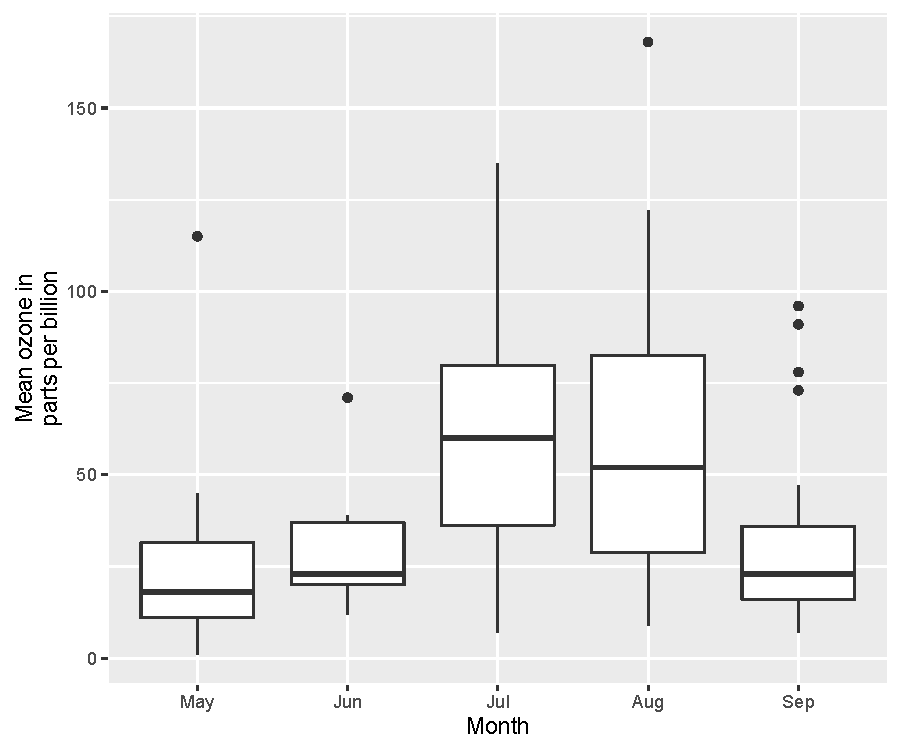
\includegraphics[width=0.6\linewidth]{10_Boxplots_pdf/box_3-1} \end{center}

\section{Changing axis ticks}\label{changing-axis-ticks}

The next thing we will change is the axis ticks. Let's make the y-axis
ticks appear at every 25 units rather than 50 using the
\texttt{breaks\ =\ seq(0,\ 175,\ 25)} argument in
\texttt{scale\_y\_continuous}. (The \texttt{seq} function is a base R
function that indicates the start and endpoints and the units to
increment by respectively. See \texttt{help(seq)} for more information.)
We ensure that the y-axis begins and ends where we want by also adding
the argument \texttt{limits\ =\ c(0,\ 175)} to
\texttt{scale\_y\_continuous}.

\begin{Shaded}
\begin{Highlighting}[]
\NormalTok{p10 <-}\StringTok{ }\NormalTok{p10 +}\StringTok{ }\KeywordTok{scale_y_continuous}\NormalTok{(}\DataTypeTok{name =} \StringTok{"Mean ozone in}\CharTok{\textbackslash{}n}\StringTok{parts per billion"}\NormalTok{,}
    \DataTypeTok{breaks =} \KeywordTok{seq}\NormalTok{(}\DecValTok{0}\NormalTok{, }\DecValTok{175}\NormalTok{, }\DecValTok{25}\NormalTok{), }\DataTypeTok{limits=}\KeywordTok{c}\NormalTok{(}\DecValTok{0}\NormalTok{, }\DecValTok{175}\NormalTok{))}
\NormalTok{p10}
\end{Highlighting}
\end{Shaded}

\begin{center}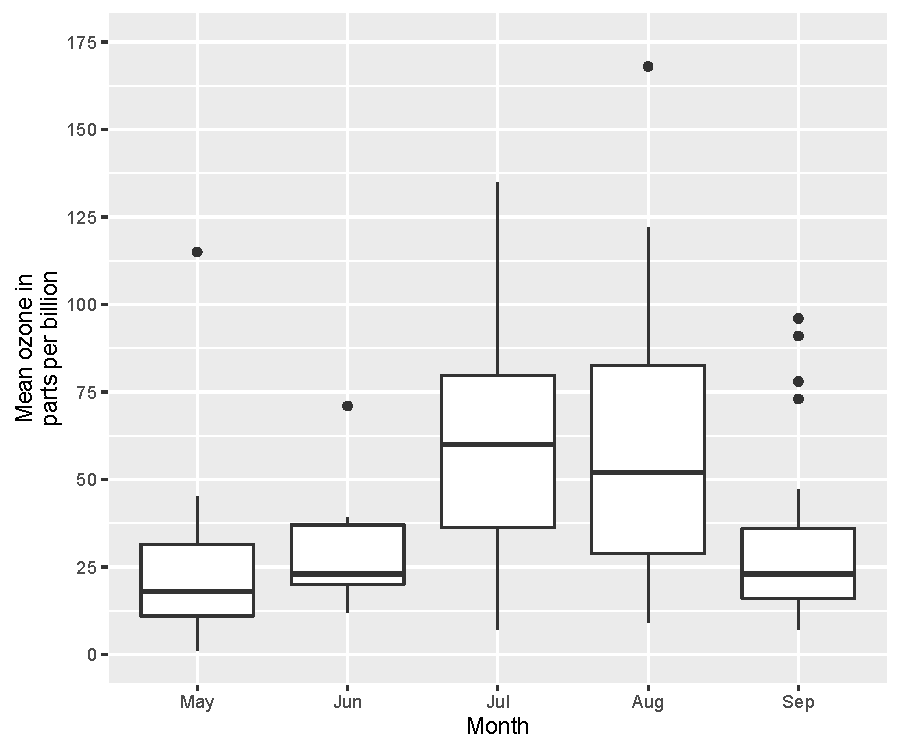
\includegraphics[width=0.6\linewidth]{10_Boxplots_pdf/box_4-1} \end{center}

\section{Adding a title}\label{adding-a-title}

To add a title, we include the option \texttt{ggtitle} and include the
name of the graph as a string argument.

\begin{Shaded}
\begin{Highlighting}[]
\NormalTok{p10 <-}\StringTok{ }\NormalTok{p10 +}\StringTok{ }\KeywordTok{ggtitle}\NormalTok{(}\StringTok{"Boxplot of mean ozone by month"}\NormalTok{)}
\NormalTok{p10}
\end{Highlighting}
\end{Shaded}

\begin{center}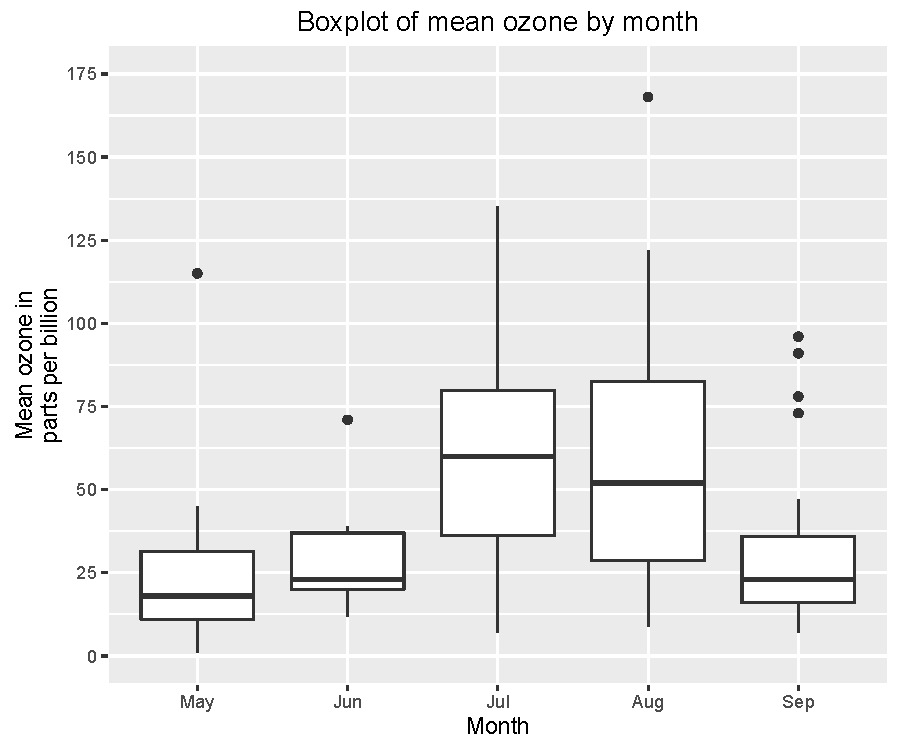
\includegraphics[width=0.6\linewidth]{10_Boxplots_pdf/box_5-1} \end{center}

\section{Changing the colour of the
boxes}\label{changing-the-colour-of-the-boxes}

To change the line and fill colours of the box plot, we add a valid
colour to the \texttt{colour} and \texttt{fill} arguments in
\texttt{geom\_boxplot()} (note that we assigned these colours to
variables outside of the plot to make it easier to change them). A list
of valid colours is
\href{http://www.stat.columbia.edu/~tzheng/files/Rcolor.pdf}{here}.

\begin{Shaded}
\begin{Highlighting}[]
\NormalTok{fill <-}\StringTok{ "gold1"}\NormalTok{; line <-}\StringTok{ "goldenrod2"}

\NormalTok{p10 <-}\StringTok{ }\KeywordTok{ggplot}\NormalTok{(airquality, }\KeywordTok{aes}\NormalTok{(}\DataTypeTok{x =} \NormalTok{Month, }\DataTypeTok{y =} \NormalTok{Ozone)) +}\StringTok{ }
\StringTok{  }\KeywordTok{geom_boxplot}\NormalTok{(}\DataTypeTok{fill =} \NormalTok{fill, }\DataTypeTok{colour =} \NormalTok{line) +}
\StringTok{  }\KeywordTok{scale_y_continuous}\NormalTok{(}\DataTypeTok{name =} \StringTok{"Mean ozone in}\CharTok{\textbackslash{}n}\StringTok{parts per billion"}\NormalTok{,}
    \DataTypeTok{breaks =} \KeywordTok{seq}\NormalTok{(}\DecValTok{0}\NormalTok{, }\DecValTok{175}\NormalTok{, }\DecValTok{25}\NormalTok{), }\DataTypeTok{limits=}\KeywordTok{c}\NormalTok{(}\DecValTok{0}\NormalTok{, }\DecValTok{175}\NormalTok{)) +}
\StringTok{  }\KeywordTok{scale_x_discrete}\NormalTok{(}\DataTypeTok{name =} \StringTok{"Month"}\NormalTok{) +}
\StringTok{  }\KeywordTok{ggtitle}\NormalTok{(}\StringTok{"Boxplot of mean ozone by month"}\NormalTok{)}
\NormalTok{p10}
\end{Highlighting}
\end{Shaded}

\begin{center}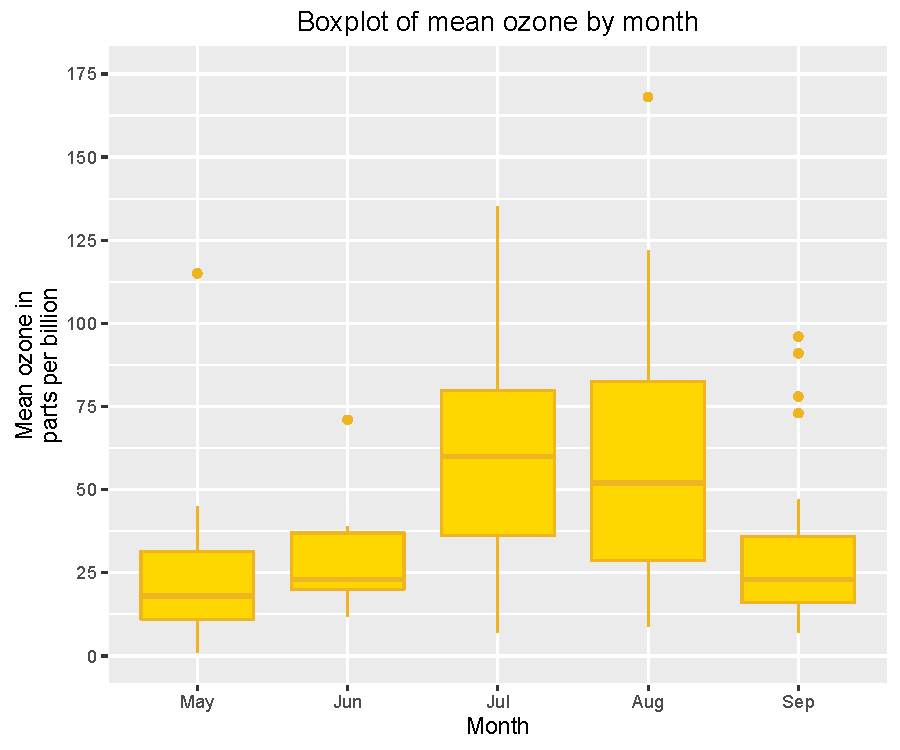
\includegraphics[width=0.6\linewidth]{10_Boxplots_pdf/box_6-1} \end{center}

If you want to go beyond the options in the list above, you can also
specify exact HEX colours by including them as a string preceded by a
hash, e.g., ``\#FFFFFF''. Below, we have called two shades of blue for
the fill and lines using their HEX codes.

\begin{Shaded}
\begin{Highlighting}[]
\NormalTok{fill <-}\StringTok{ "#4271AE"}\NormalTok{; line <-}\StringTok{ "#1F3552"}

\NormalTok{p10 <-}\StringTok{ }\KeywordTok{ggplot}\NormalTok{(airquality, }\KeywordTok{aes}\NormalTok{(}\DataTypeTok{x =} \NormalTok{Month, }\DataTypeTok{y =} \NormalTok{Ozone)) +}\StringTok{ }
\StringTok{  }\KeywordTok{geom_boxplot}\NormalTok{(}\DataTypeTok{fill =} \NormalTok{fill, }\DataTypeTok{colour =} \NormalTok{line) +}
\StringTok{  }\KeywordTok{scale_y_continuous}\NormalTok{(}\DataTypeTok{name =} \StringTok{"Mean ozone in}\CharTok{\textbackslash{}n}\StringTok{parts per billion"}\NormalTok{,}
    \DataTypeTok{breaks =} \KeywordTok{seq}\NormalTok{(}\DecValTok{0}\NormalTok{, }\DecValTok{175}\NormalTok{, }\DecValTok{25}\NormalTok{), }\DataTypeTok{limits=}\KeywordTok{c}\NormalTok{(}\DecValTok{0}\NormalTok{, }\DecValTok{175}\NormalTok{)) +}
\StringTok{  }\KeywordTok{scale_x_discrete}\NormalTok{(}\DataTypeTok{name =} \StringTok{"Month"}\NormalTok{) +}
\StringTok{  }\KeywordTok{ggtitle}\NormalTok{(}\StringTok{"Boxplot of mean ozone by month"}\NormalTok{)}
\NormalTok{p10}
\end{Highlighting}
\end{Shaded}

\begin{center}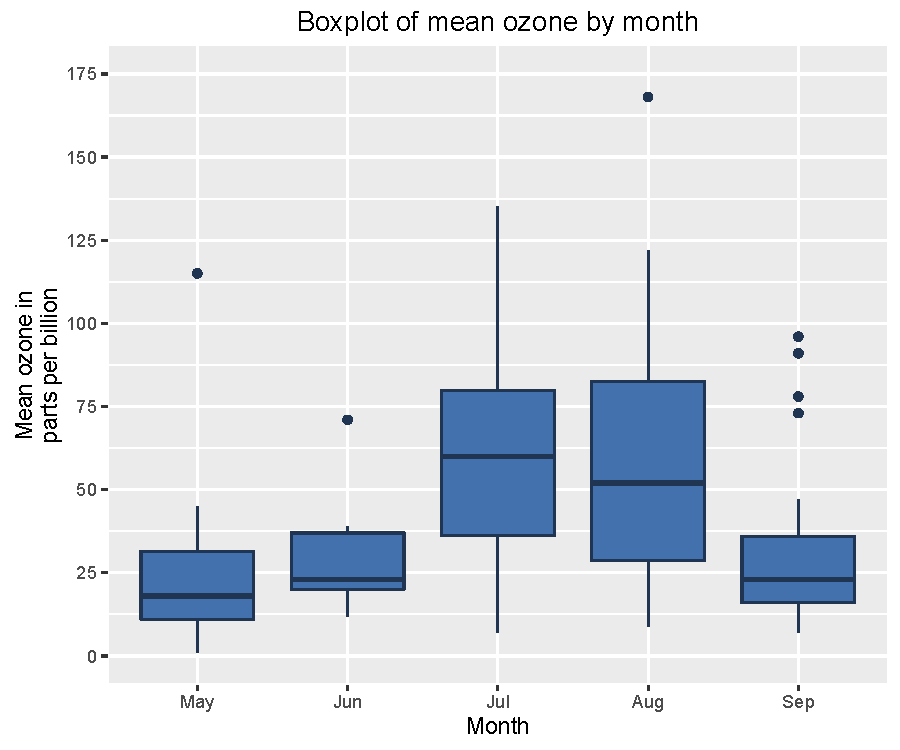
\includegraphics[width=0.6\linewidth]{10_Boxplots_pdf/box_7-1} \end{center}

You can also specify the degree of transparency in the box fill area
using the argument \texttt{alpha} in \texttt{geom\_boxplot}. This ranges
from 0 to 1.

\begin{Shaded}
\begin{Highlighting}[]
\NormalTok{p10 <-}\StringTok{ }\KeywordTok{ggplot}\NormalTok{(airquality, }\KeywordTok{aes}\NormalTok{(}\DataTypeTok{x =} \NormalTok{Month, }\DataTypeTok{y =} \NormalTok{Ozone)) +}\StringTok{ }
\StringTok{  }\KeywordTok{geom_boxplot}\NormalTok{(}\DataTypeTok{fill =} \NormalTok{fill, }\DataTypeTok{colour =} \NormalTok{line, }\DataTypeTok{alpha =} \FloatTok{0.7}\NormalTok{) +}
\StringTok{  }\KeywordTok{scale_y_continuous}\NormalTok{(}\DataTypeTok{name =} \StringTok{"Mean ozone in}\CharTok{\textbackslash{}n}\StringTok{parts per billion"}\NormalTok{,}
    \DataTypeTok{breaks =} \KeywordTok{seq}\NormalTok{(}\DecValTok{0}\NormalTok{, }\DecValTok{175}\NormalTok{, }\DecValTok{25}\NormalTok{), }\DataTypeTok{limits=}\KeywordTok{c}\NormalTok{(}\DecValTok{0}\NormalTok{, }\DecValTok{175}\NormalTok{)) +}
\StringTok{  }\KeywordTok{scale_x_discrete}\NormalTok{(}\DataTypeTok{name =} \StringTok{"Month"}\NormalTok{) +}
\StringTok{  }\KeywordTok{ggtitle}\NormalTok{(}\StringTok{"Boxplot of mean ozone by month"}\NormalTok{)}
\NormalTok{p10}
\end{Highlighting}
\end{Shaded}

\begin{center}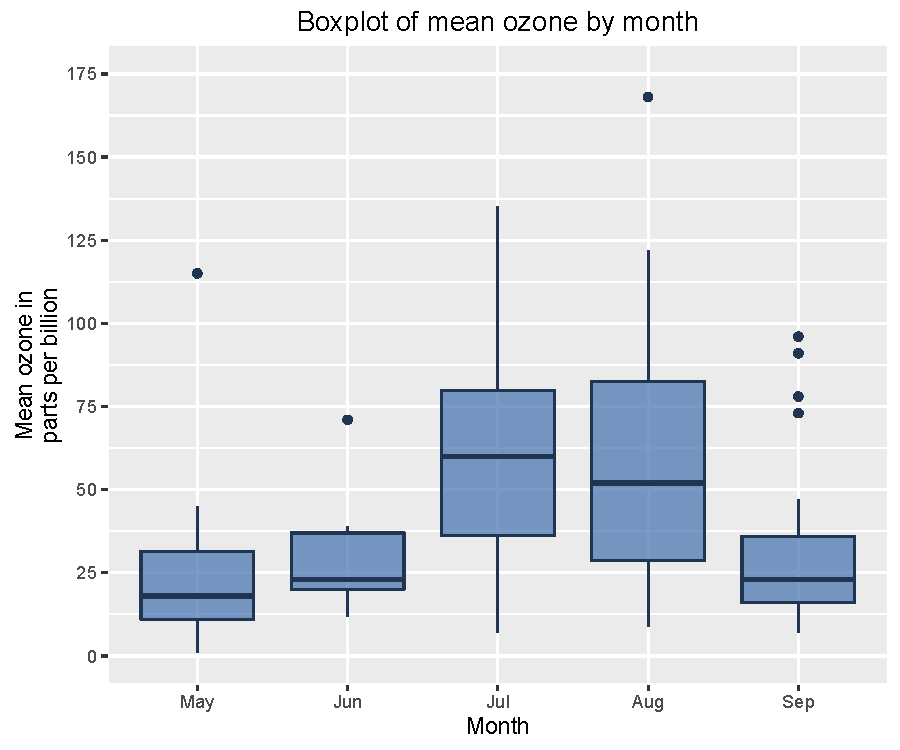
\includegraphics[width=0.6\linewidth]{10_Boxplots_pdf/box_8-1} \end{center}

Finally, you can change the appearance of the outliers as well, using
the arguments \texttt{outlier.colour} and \texttt{outlier.shape} in
\texttt{geom\_boxplot} to change the colour and shape respectively. An
explanation of the allowed arguments for shape are described in
\href{http://sape.inf.usi.ch/quick-reference/ggplot2/shape}{this
article}, although be aware that because there is no ``fill'' argument
for outlier, you cannot create circles with separate outline and fill
colours. Here we will make the outliers small solid circles (using
\texttt{outlier.shape\ =\ 20}) and make them the same colour as the box
lines (using \texttt{outlier.colour\ =\ "\#1F3552"}).

\begin{Shaded}
\begin{Highlighting}[]
\NormalTok{p10 <-}\StringTok{ }\KeywordTok{ggplot}\NormalTok{(airquality, }\KeywordTok{aes}\NormalTok{(}\DataTypeTok{x =} \NormalTok{Month, }\DataTypeTok{y =} \NormalTok{Ozone)) +}\StringTok{ }
\StringTok{  }\KeywordTok{geom_boxplot}\NormalTok{(}\DataTypeTok{fill =} \NormalTok{fill, }\DataTypeTok{colour =} \NormalTok{line, }\DataTypeTok{alpha =} \FloatTok{0.7}\NormalTok{,}
    \DataTypeTok{outlier.colour =} \StringTok{"#1F3552"}\NormalTok{, }\DataTypeTok{outlier.shape =} \DecValTok{20}\NormalTok{) +}
\StringTok{  }\KeywordTok{scale_y_continuous}\NormalTok{(}\DataTypeTok{name =} \StringTok{"Mean ozone in}\CharTok{\textbackslash{}n}\StringTok{parts per billion"}\NormalTok{,}
    \DataTypeTok{breaks =} \KeywordTok{seq}\NormalTok{(}\DecValTok{0}\NormalTok{, }\DecValTok{175}\NormalTok{, }\DecValTok{25}\NormalTok{), }\DataTypeTok{limits=}\KeywordTok{c}\NormalTok{(}\DecValTok{0}\NormalTok{, }\DecValTok{175}\NormalTok{)) +}
\StringTok{  }\KeywordTok{scale_x_discrete}\NormalTok{(}\DataTypeTok{name =} \StringTok{"Month"}\NormalTok{) +}
\StringTok{  }\KeywordTok{ggtitle}\NormalTok{(}\StringTok{"Boxplot of mean ozone by month"}\NormalTok{)}
\NormalTok{p10}
\end{Highlighting}
\end{Shaded}

\begin{center}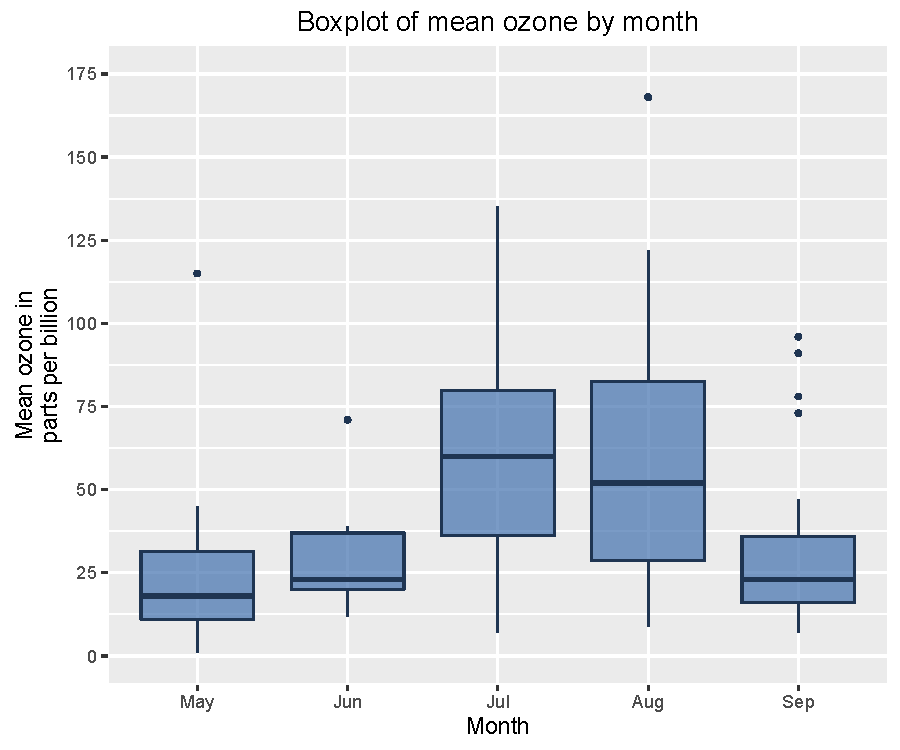
\includegraphics[width=0.6\linewidth]{10_Boxplots_pdf/box_9-1} \end{center}

\section{Using the white theme}\label{using-the-white-theme}

As explained in the previous posts, we can also change the overall look
of the plot using themes. We'll start using a simple theme customisation
by adding \texttt{theme\_bw()}. As you can see, we can further tweak the
graph using the \texttt{theme} option, which we've used so far to change
the legend.

\begin{Shaded}
\begin{Highlighting}[]
\NormalTok{p10 <-}\StringTok{ }\NormalTok{p10 +}\StringTok{ }\KeywordTok{theme_bw}\NormalTok{()}
\NormalTok{p10}
\end{Highlighting}
\end{Shaded}

\begin{center}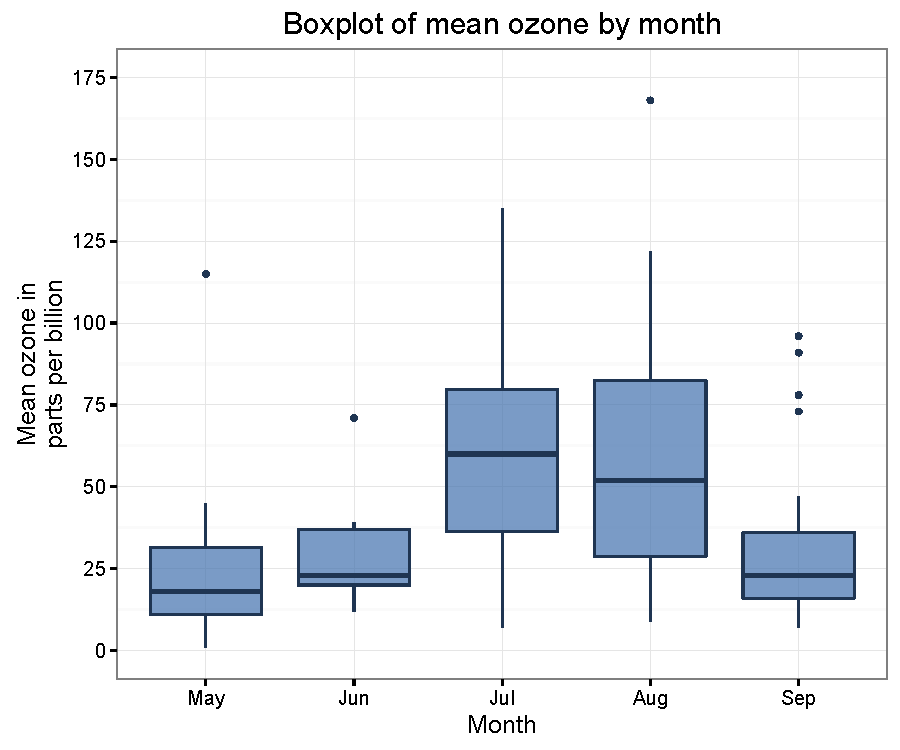
\includegraphics[width=0.6\linewidth]{10_Boxplots_pdf/box_10-1} \end{center}

\section{Creating an XKCD style
chart}\label{creating-an-xkcd-style-chart}

Of course, you may want to create your own themes as well.
\texttt{ggplot2} allows for a very high degree of customisation,
including allowing you to use imported fonts. Below is an example of a
theme Mauricio was able to create which mimics the visual style of
\href{http://xkcd.com/}{XKCD}. In order to create this chart, you first
need to import the XKCD font, and load it into R using the
\texttt{extrafont} package.

\begin{Shaded}
\begin{Highlighting}[]
\NormalTok{p10 <-}\StringTok{ }\KeywordTok{ggplot}\NormalTok{(airquality, }\KeywordTok{aes}\NormalTok{(}\DataTypeTok{x =} \NormalTok{Month, }\DataTypeTok{y =} \NormalTok{Ozone)) +}\StringTok{ }
\StringTok{  }\KeywordTok{geom_boxplot}\NormalTok{(}\DataTypeTok{colour =} \StringTok{"black"}\NormalTok{, }\DataTypeTok{fill =} \StringTok{"#56B4E9"}\NormalTok{) +}
\StringTok{  }\KeywordTok{scale_y_continuous}\NormalTok{(}\DataTypeTok{name =} \StringTok{"Mean ozone in}\CharTok{\textbackslash{}n}\StringTok{parts per billion"}\NormalTok{,}
    \DataTypeTok{breaks =} \KeywordTok{seq}\NormalTok{(}\DecValTok{0}\NormalTok{, }\DecValTok{175}\NormalTok{, }\DecValTok{25}\NormalTok{), }\DataTypeTok{limits=}\KeywordTok{c}\NormalTok{(}\DecValTok{0}\NormalTok{, }\DecValTok{175}\NormalTok{)) +}
\StringTok{  }\KeywordTok{scale_x_discrete}\NormalTok{(}\DataTypeTok{name =} \StringTok{"Month"}\NormalTok{) +}
\StringTok{  }\KeywordTok{ggtitle}\NormalTok{(}\StringTok{"Boxplot of mean ozone by month"}\NormalTok{) +}
\StringTok{  }\KeywordTok{theme}\NormalTok{(}\DataTypeTok{axis.line.x =} \KeywordTok{element_line}\NormalTok{(}\DataTypeTok{size=}\NormalTok{.}\DecValTok{5}\NormalTok{, }\DataTypeTok{colour =} \StringTok{"black"}\NormalTok{), }
    \DataTypeTok{axis.line.y =} \KeywordTok{element_line}\NormalTok{(}\DataTypeTok{size=}\NormalTok{.}\DecValTok{5}\NormalTok{, }\DataTypeTok{colour =} \StringTok{"black"}\NormalTok{),     }
    \DataTypeTok{axis.text.x=}\KeywordTok{element_text}\NormalTok{(}\DataTypeTok{colour=}\StringTok{"black"}\NormalTok{, }\DataTypeTok{size =} \DecValTok{10}\NormalTok{), }
    \DataTypeTok{axis.text.y=}\KeywordTok{element_text}\NormalTok{(}\DataTypeTok{colour=}\StringTok{"black"}\NormalTok{, }\DataTypeTok{size =} \DecValTok{10}\NormalTok{), }
    \DataTypeTok{legend.position=}\StringTok{"bottom"}\NormalTok{, }
    \DataTypeTok{legend.direction=}\StringTok{"horizontal"}\NormalTok{,}
    \DataTypeTok{legend.box =} \StringTok{"horizontal"}\NormalTok{, }
    \DataTypeTok{legend.key =} \KeywordTok{element_blank}\NormalTok{(),}
    \DataTypeTok{panel.grid.major =} \KeywordTok{element_blank}\NormalTok{(),}
    \DataTypeTok{panel.grid.minor =} \KeywordTok{element_blank}\NormalTok{(), }
    \DataTypeTok{panel.border =} \KeywordTok{element_blank}\NormalTok{(),}
    \DataTypeTok{panel.background =} \KeywordTok{element_blank}\NormalTok{(),}
    \DataTypeTok{plot.title=}\KeywordTok{element_text}\NormalTok{(}\DataTypeTok{family=}\StringTok{"xkcd-Regular"}\NormalTok{), }
    \DataTypeTok{text=}\KeywordTok{element_text}\NormalTok{(}\DataTypeTok{family=}\StringTok{"xkcd-Regular"}\NormalTok{)) }
\NormalTok{p10}
\end{Highlighting}
\end{Shaded}

\begin{center}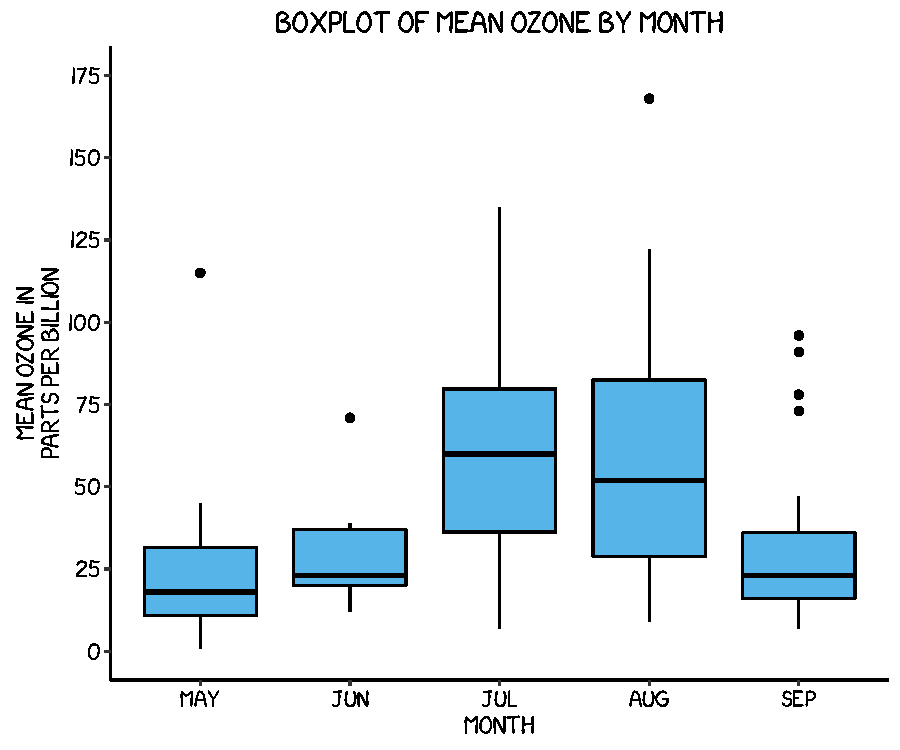
\includegraphics[width=0.6\linewidth]{10_Boxplots_pdf/box_11-1} \end{center}

\section{\texorpdfstring{Using `The Economist'
theme}{Using The Economist theme}}\label{using-the-economist-theme}

There are a wider range of pre-built themes available as part of the
\texttt{ggthemes} package (more information on these
\href{https://cran.r-project.org/web/packages/ggthemes/vignettes/ggthemes.html}{here}).
Below we've applied \texttt{theme\_economist()}, which approximates
graphs in the Economist magazine.

\begin{Shaded}
\begin{Highlighting}[]
\NormalTok{p10 <-}\StringTok{ }\KeywordTok{ggplot}\NormalTok{(airquality, }\KeywordTok{aes}\NormalTok{(}\DataTypeTok{x =} \NormalTok{Month, }\DataTypeTok{y =} \NormalTok{Ozone)) +}\StringTok{ }
\StringTok{  }\KeywordTok{geom_boxplot}\NormalTok{(}\DataTypeTok{fill =} \NormalTok{fill, }\DataTypeTok{colour =} \NormalTok{line) +}
\StringTok{  }\KeywordTok{scale_y_continuous}\NormalTok{(}\DataTypeTok{name =} \StringTok{"Mean ozone in}\CharTok{\textbackslash{}n}\StringTok{parts per billion"}\NormalTok{,}
    \DataTypeTok{breaks =} \KeywordTok{seq}\NormalTok{(}\DecValTok{0}\NormalTok{, }\DecValTok{175}\NormalTok{, }\DecValTok{25}\NormalTok{), }\DataTypeTok{limits=}\KeywordTok{c}\NormalTok{(}\DecValTok{0}\NormalTok{, }\DecValTok{175}\NormalTok{)) +}
\StringTok{  }\KeywordTok{scale_x_discrete}\NormalTok{(}\DataTypeTok{name =} \StringTok{"Month"}\NormalTok{) +}
\StringTok{  }\KeywordTok{ggtitle}\NormalTok{(}\StringTok{"Boxplot of mean ozone by month"}\NormalTok{) +}
\StringTok{  }\KeywordTok{theme_economist}\NormalTok{() +}\StringTok{ }\KeywordTok{scale_fill_economist}\NormalTok{() +}
\StringTok{  }\KeywordTok{theme}\NormalTok{(}\DataTypeTok{axis.line.x =} \KeywordTok{element_line}\NormalTok{(}\DataTypeTok{size=}\NormalTok{.}\DecValTok{5}\NormalTok{, }\DataTypeTok{colour =} \StringTok{"black"}\NormalTok{),}
    \DataTypeTok{axis.title =} \KeywordTok{element_text}\NormalTok{(}\DataTypeTok{size =} \DecValTok{12}\NormalTok{),}
    \DataTypeTok{legend.position=}\StringTok{"bottom"}\NormalTok{, }
    \DataTypeTok{legend.direction=}\StringTok{"horizontal"}\NormalTok{,}
    \DataTypeTok{legend.box =} \StringTok{"horizontal"}\NormalTok{, }
    \DataTypeTok{legend.text =} \KeywordTok{element_text}\NormalTok{(}\DataTypeTok{size =} \DecValTok{10}\NormalTok{),}
    \DataTypeTok{text =} \KeywordTok{element_text}\NormalTok{(}\DataTypeTok{family =} \StringTok{"OfficinaSanITC-Book"}\NormalTok{),}
    \DataTypeTok{plot.title =} \KeywordTok{element_text}\NormalTok{(}\DataTypeTok{family=}\StringTok{"OfficinaSanITC-Book"}\NormalTok{))}
\NormalTok{p10}
\end{Highlighting}
\end{Shaded}

\begin{center}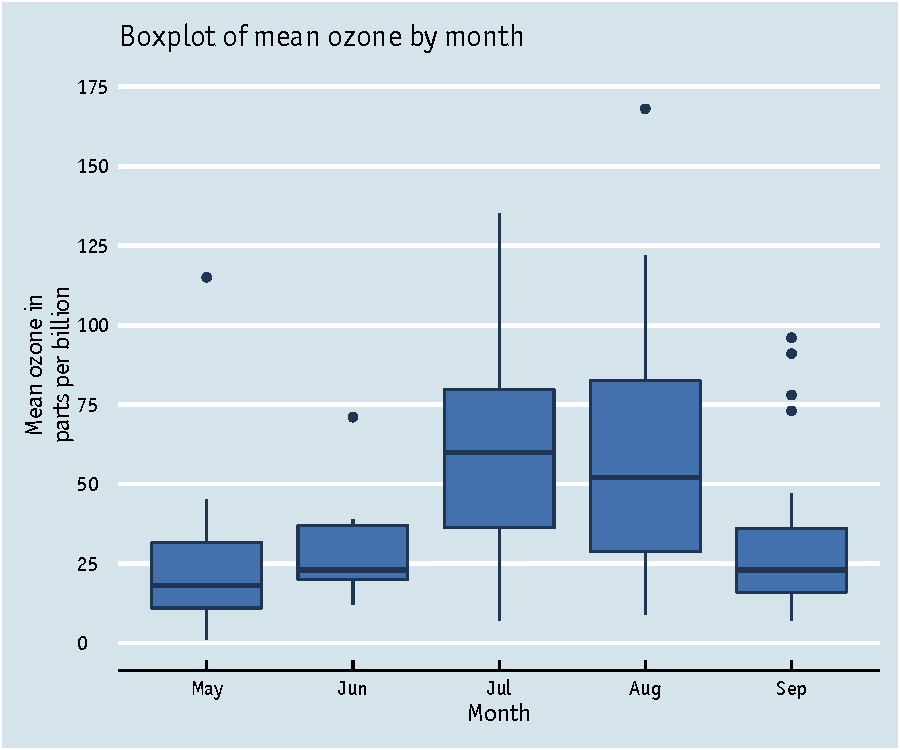
\includegraphics[width=0.6\linewidth]{10_Boxplots_pdf/box_12-1} \end{center}

\section{\texorpdfstring{Using `Five Thirty Eight'
theme}{Using Five Thirty Eight theme}}\label{using-five-thirty-eight-theme}

Below we've applied \texttt{theme\_fivethirtyeight()}, which
approximates graphs in the nice
\href{http://fivethirtyeight.com/}{FiveThirtyEight} website. Again, it
is also important that the font change is optional and it's only to
obtain a more similar result compared to the original. For an exact
result you need `Atlas Grotesk' and `Decima Mono Pro' which are
commercial font and are available
\href{https://commercialtype.com/catalog/atlas}{here} and
\href{https://www.myfonts.com/fonts/tipografiaramis/decima-mono-pro/}{here}.

\begin{Shaded}
\begin{Highlighting}[]
\NormalTok{p10 <-}\StringTok{ }\KeywordTok{ggplot}\NormalTok{(airquality, }\KeywordTok{aes}\NormalTok{(}\DataTypeTok{x =} \NormalTok{Month, }\DataTypeTok{y =} \NormalTok{Ozone)) +}\StringTok{ }
\StringTok{  }\KeywordTok{geom_boxplot}\NormalTok{(}\DataTypeTok{fill =} \NormalTok{fill, }\DataTypeTok{colour =} \NormalTok{line) +}
\StringTok{  }\KeywordTok{scale_y_continuous}\NormalTok{(}\DataTypeTok{name =} \StringTok{"Mean ozone in}\CharTok{\textbackslash{}n}\StringTok{parts per billion"}\NormalTok{,}
    \DataTypeTok{breaks =} \KeywordTok{seq}\NormalTok{(}\DecValTok{0}\NormalTok{, }\DecValTok{175}\NormalTok{, }\DecValTok{25}\NormalTok{), }\DataTypeTok{limits=}\KeywordTok{c}\NormalTok{(}\DecValTok{0}\NormalTok{, }\DecValTok{175}\NormalTok{)) +}
\StringTok{  }\KeywordTok{scale_x_discrete}\NormalTok{(}\DataTypeTok{name =} \StringTok{"Month"}\NormalTok{) +}
\StringTok{  }\KeywordTok{ggtitle}\NormalTok{(}\StringTok{"Boxplot of mean ozone by month"}\NormalTok{) +}
\StringTok{  }\KeywordTok{theme_fivethirtyeight}\NormalTok{() +}\StringTok{ }\KeywordTok{scale_fill_fivethirtyeight}\NormalTok{() +}\StringTok{   }
\StringTok{  }\KeywordTok{theme}\NormalTok{(}\DataTypeTok{axis.title =} \KeywordTok{element_text}\NormalTok{(}\DataTypeTok{family=}\StringTok{"Atlas Grotesk Regular"}\NormalTok{),}
    \DataTypeTok{legend.position=}\StringTok{"bottom"}\NormalTok{, }
    \DataTypeTok{legend.direction=}\StringTok{"horizontal"}\NormalTok{,}
    \DataTypeTok{legend.box =} \StringTok{"horizontal"}\NormalTok{, }
    \DataTypeTok{legend.title=}\KeywordTok{element_text}\NormalTok{(}\DataTypeTok{family=}\StringTok{"Atlas Grotesk Regular"}\NormalTok{, }\DataTypeTok{size =} \DecValTok{10}\NormalTok{),}
    \DataTypeTok{legend.text=}\KeywordTok{element_text}\NormalTok{(}\DataTypeTok{family=}\StringTok{"Atlas Grotesk Regular"}\NormalTok{, }\DataTypeTok{size =} \DecValTok{10}\NormalTok{),}
    \DataTypeTok{plot.title=}\KeywordTok{element_text}\NormalTok{(}\DataTypeTok{family=}\StringTok{"Atlas Grotesk Medium"}\NormalTok{), }
    \DataTypeTok{text=}\KeywordTok{element_text}\NormalTok{(}\DataTypeTok{family=}\StringTok{"DecimaMonoPro"}\NormalTok{)) }
\NormalTok{p10}
\end{Highlighting}
\end{Shaded}

\begin{center}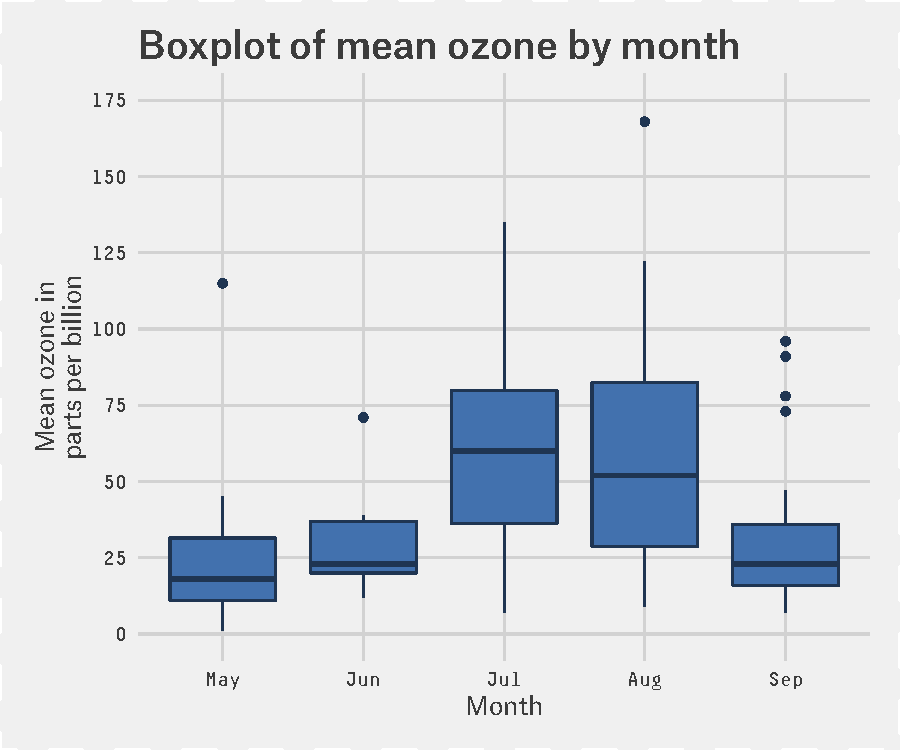
\includegraphics[width=0.6\linewidth]{10_Boxplots_pdf/box_13-1} \end{center}

\section{Creating your own theme}\label{creating-your-own-theme}

As before, you can modify your plots a lot as \texttt{ggplot2} allows
many customisations. Here is a custom plot where we have modified the
axes, background and font.

\begin{Shaded}
\begin{Highlighting}[]
\NormalTok{fill <-}\StringTok{ "#4271AE"}\NormalTok{; lines <-}\StringTok{ "#1F3552"}

\NormalTok{p10 <-}\StringTok{ }\KeywordTok{ggplot}\NormalTok{(airquality, }\KeywordTok{aes}\NormalTok{(}\DataTypeTok{x =} \NormalTok{Month, }\DataTypeTok{y =} \NormalTok{Ozone)) +}\StringTok{ }
\StringTok{  }\KeywordTok{geom_boxplot}\NormalTok{(}\DataTypeTok{colour =} \NormalTok{lines, }\DataTypeTok{fill =} \NormalTok{fill, }\DataTypeTok{size =} \DecValTok{1}\NormalTok{) +}
\StringTok{  }\KeywordTok{scale_y_continuous}\NormalTok{(}\DataTypeTok{name =} \StringTok{"Mean ozone in}\CharTok{\textbackslash{}n}\StringTok{parts per billion"}\NormalTok{,}
    \DataTypeTok{breaks =} \KeywordTok{seq}\NormalTok{(}\DecValTok{0}\NormalTok{, }\DecValTok{175}\NormalTok{, }\DecValTok{25}\NormalTok{), }\DataTypeTok{limits=}\KeywordTok{c}\NormalTok{(}\DecValTok{0}\NormalTok{, }\DecValTok{175}\NormalTok{)) +}
\StringTok{  }\KeywordTok{scale_x_discrete}\NormalTok{(}\DataTypeTok{name =} \StringTok{"Month"}\NormalTok{) +}
\StringTok{  }\KeywordTok{ggtitle}\NormalTok{(}\StringTok{"Boxplot of mean ozone by month"}\NormalTok{) +}
\StringTok{  }\KeywordTok{theme_bw}\NormalTok{() +}
\StringTok{  }\KeywordTok{theme}\NormalTok{(}\DataTypeTok{panel.border =} \KeywordTok{element_rect}\NormalTok{(}\DataTypeTok{colour =} \StringTok{"black"}\NormalTok{, }\DataTypeTok{fill=}\OtherTok{NA}\NormalTok{, }\DataTypeTok{size=}\NormalTok{.}\DecValTok{5}\NormalTok{),}
    \DataTypeTok{panel.grid.major =} \KeywordTok{element_line}\NormalTok{(}\DataTypeTok{colour =} \StringTok{"#d3d3d3"}\NormalTok{), }
    \DataTypeTok{panel.grid.minor =} \KeywordTok{element_blank}\NormalTok{(), }
    \DataTypeTok{panel.border =} \KeywordTok{element_blank}\NormalTok{(), }\DataTypeTok{panel.background =} \KeywordTok{element_blank}\NormalTok{(),}
    \DataTypeTok{plot.title =} \KeywordTok{element_text}\NormalTok{(}\DataTypeTok{size =} \DecValTok{14}\NormalTok{, }\DataTypeTok{family =} \StringTok{"Tahoma"}\NormalTok{, }\DataTypeTok{face =} \StringTok{"bold"}\NormalTok{),}
    \DataTypeTok{text=}\KeywordTok{element_text}\NormalTok{(}\DataTypeTok{family =} \StringTok{"Tahoma"}\NormalTok{), }
    \DataTypeTok{axis.title =} \KeywordTok{element_text}\NormalTok{(}\DataTypeTok{face=}\StringTok{"bold"}\NormalTok{),}
    \DataTypeTok{axis.text.x =} \KeywordTok{element_text}\NormalTok{(}\DataTypeTok{colour=}\StringTok{"black"}\NormalTok{, }\DataTypeTok{size =} \DecValTok{11}\NormalTok{),}
    \DataTypeTok{axis.text.y =} \KeywordTok{element_text}\NormalTok{(}\DataTypeTok{colour=}\StringTok{"black"}\NormalTok{, }\DataTypeTok{size =} \DecValTok{9}\NormalTok{)) }
\NormalTok{p10}
\end{Highlighting}
\end{Shaded}

\begin{center}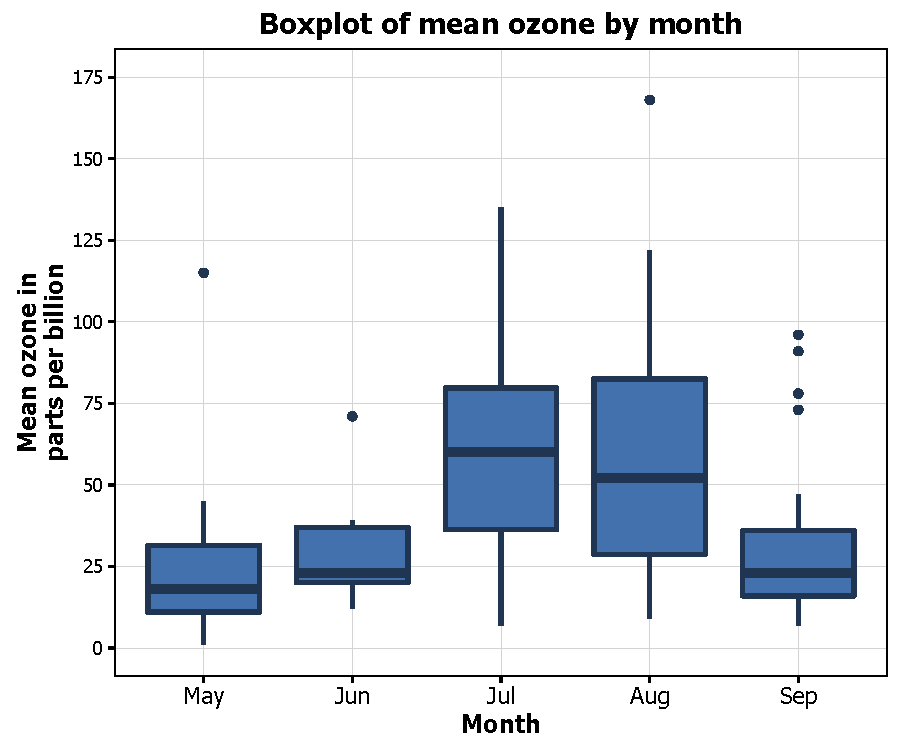
\includegraphics[width=0.6\linewidth]{10_Boxplots_pdf/box_14-1} \end{center}

\section{Boxplot extras}\label{boxplot-extras}

An extra feature you can add to boxplots is to overlay all of the points
for that group on each boxplot in order to get an idea of the sample
size of the group. This can be achieved using by adding the
\texttt{geom\_jitter} option.

\begin{Shaded}
\begin{Highlighting}[]
\NormalTok{p10 <-}\StringTok{ }\NormalTok{p10 +}\StringTok{ }\KeywordTok{geom_jitter}\NormalTok{()}
\NormalTok{p10}
\end{Highlighting}
\end{Shaded}

\begin{center}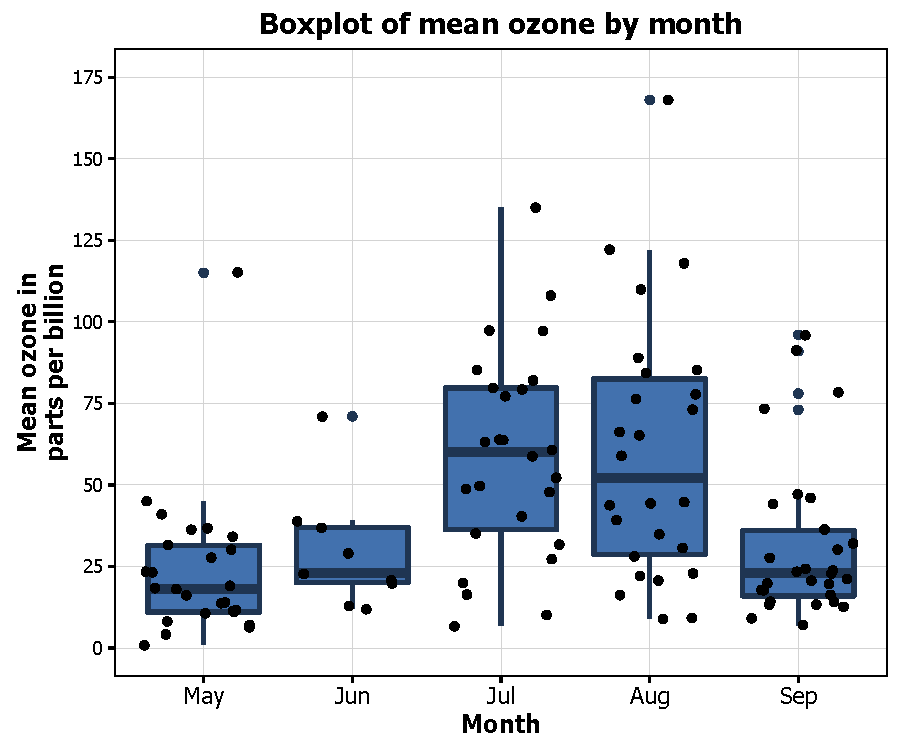
\includegraphics[width=0.6\linewidth]{10_Boxplots_pdf/box_15-1} \end{center}

We can see that June has a pretty small sample, indicating that
information based on this group may not be very reliable.

Another thing you can do with your boxplot is add a notch to the box
where the median sits to give a clearer visual indication of how the
data are distributed within the IQR. You achieve this by adding the
argument \texttt{notch\ =\ TRUE} to the \texttt{geom\_boxplot} option.
You can see on our graph that the box for June looks a bit weird due to
the very small gap between the 25th percentile and the median.

\begin{Shaded}
\begin{Highlighting}[]
\NormalTok{p10 <-}\StringTok{ }\KeywordTok{ggplot}\NormalTok{(airquality, }\KeywordTok{aes}\NormalTok{(}\DataTypeTok{x =} \NormalTok{Month, }\DataTypeTok{y =} \NormalTok{Ozone)) +}\StringTok{ }
\StringTok{  }\KeywordTok{geom_boxplot}\NormalTok{(}\DataTypeTok{colour =} \NormalTok{lines, }\DataTypeTok{fill =} \NormalTok{fill, }\DataTypeTok{size =} \DecValTok{1}\NormalTok{, }\DataTypeTok{notch =} \OtherTok{TRUE}\NormalTok{) +}
\StringTok{  }\KeywordTok{scale_y_continuous}\NormalTok{(}\DataTypeTok{name =} \StringTok{"Mean ozone in}\CharTok{\textbackslash{}n}\StringTok{parts per billion"}\NormalTok{,}
    \DataTypeTok{breaks =} \KeywordTok{seq}\NormalTok{(}\DecValTok{0}\NormalTok{, }\DecValTok{175}\NormalTok{, }\DecValTok{25}\NormalTok{), }\DataTypeTok{limits=}\KeywordTok{c}\NormalTok{(}\DecValTok{0}\NormalTok{, }\DecValTok{175}\NormalTok{)) +}
\StringTok{  }\KeywordTok{scale_x_discrete}\NormalTok{(}\DataTypeTok{name =} \StringTok{"Month"}\NormalTok{) +}
\StringTok{  }\KeywordTok{ggtitle}\NormalTok{(}\StringTok{"Boxplot of mean ozone by month"}\NormalTok{) +}
\StringTok{  }\KeywordTok{theme_bw}\NormalTok{() +}
\StringTok{  }\KeywordTok{theme}\NormalTok{(}\DataTypeTok{panel.border =} \KeywordTok{element_rect}\NormalTok{(}\DataTypeTok{colour =} \StringTok{"black"}\NormalTok{, }\DataTypeTok{fill=}\OtherTok{NA}\NormalTok{, }\DataTypeTok{size=}\NormalTok{.}\DecValTok{5}\NormalTok{),}
    \DataTypeTok{panel.grid.major =} \KeywordTok{element_line}\NormalTok{(}\DataTypeTok{colour =} \StringTok{"#d3d3d3"}\NormalTok{), }
    \DataTypeTok{panel.grid.minor =} \KeywordTok{element_blank}\NormalTok{(), }
    \DataTypeTok{panel.border =} \KeywordTok{element_blank}\NormalTok{(), }\DataTypeTok{panel.background =} \KeywordTok{element_blank}\NormalTok{(),}
    \DataTypeTok{plot.title =} \KeywordTok{element_text}\NormalTok{(}\DataTypeTok{size =} \DecValTok{14}\NormalTok{, }\DataTypeTok{family =} \StringTok{"Tahoma"}\NormalTok{, }\DataTypeTok{face =} \StringTok{"bold"}\NormalTok{),}
    \DataTypeTok{text=}\KeywordTok{element_text}\NormalTok{(}\DataTypeTok{family=}\StringTok{"Tahoma"}\NormalTok{), }
    \DataTypeTok{axis.title =} \KeywordTok{element_text}\NormalTok{(}\DataTypeTok{face=}\StringTok{"bold"}\NormalTok{),}
    \DataTypeTok{axis.text.x=}\KeywordTok{element_text}\NormalTok{(}\DataTypeTok{colour=}\StringTok{"black"}\NormalTok{, }\DataTypeTok{size =} \DecValTok{11}\NormalTok{), }
    \DataTypeTok{axis.text.y=}\KeywordTok{element_text}\NormalTok{(}\DataTypeTok{colour=}\StringTok{"black"}\NormalTok{, }\DataTypeTok{size =} \DecValTok{9}\NormalTok{)) }
\NormalTok{p10}
\end{Highlighting}
\end{Shaded}

\begin{center}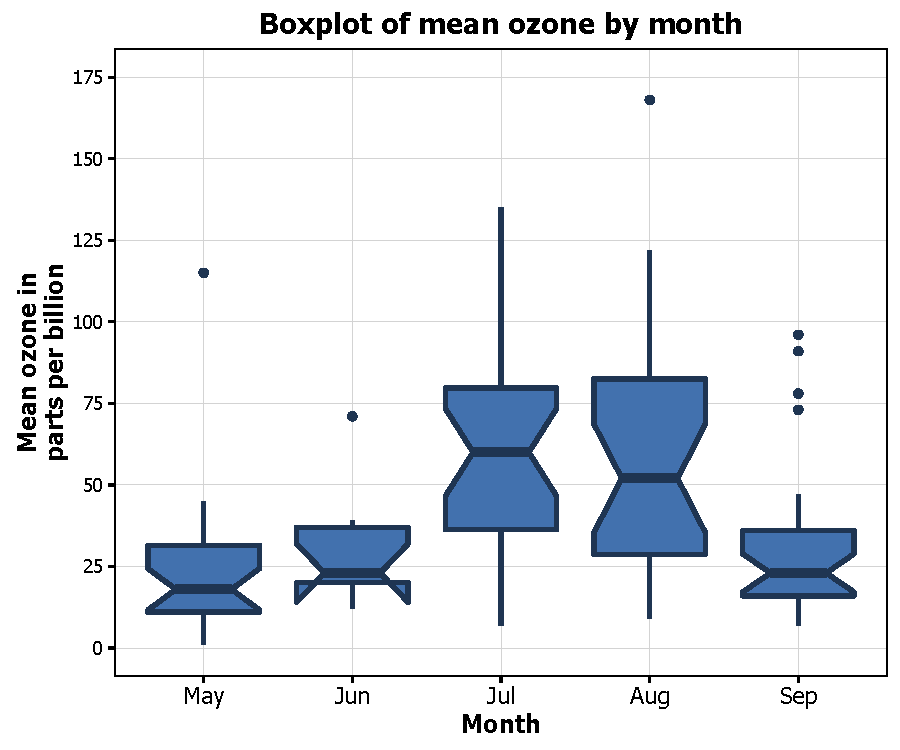
\includegraphics[width=0.6\linewidth]{10_Boxplots_pdf/box_16-1} \end{center}

\section{Grouping by another
variable}\label{grouping-by-another-variable}

You can also easily group box plots by the levels of another variable.
There are two options, in separate (panel) plots, or in the same plot.

We first need to do a little data wrangling. In order to make the graphs
a bit clearer, we've kept only months ``July'', ``Aug'' and ``Sep'' in a
new dataset \texttt{airquality\_trimmed}. We've also mean-split
\texttt{Temp} so that this is also categorical, and made it into a new
labelled factor variable called \texttt{Temp.f}.

In order to produce a panel plot by Temperature , we add the
\texttt{facet\_grid(.\ \textasciitilde{}\ Temp.f)} option to the plot.

\begin{Shaded}
\begin{Highlighting}[]
\NormalTok{airquality_trimmed <-}\StringTok{ }\NormalTok{airquality[}\KeywordTok{which}\NormalTok{(airquality$Month ==}\StringTok{ "Jul"} \NormalTok{|}
\StringTok{    }\NormalTok{airquality$Month ==}\StringTok{ "Aug"} \NormalTok{|}\StringTok{ }\NormalTok{airquality$Month ==}\StringTok{ "Sep"}\NormalTok{), ]}
\NormalTok{airquality_trimmed$Temp.f <-}\StringTok{ }\KeywordTok{factor}\NormalTok{(}\KeywordTok{ifelse}\NormalTok{(airquality_trimmed$Temp >}\StringTok{ }
\StringTok{    }\KeywordTok{mean}\NormalTok{(airquality_trimmed$Temp), }\DecValTok{1}\NormalTok{, }\DecValTok{0}\NormalTok{), }\DataTypeTok{labels =} \KeywordTok{c}\NormalTok{(}\StringTok{"Low temp "}\NormalTok{, }\StringTok{"High temp "}\NormalTok{))}

\NormalTok{p10 <-}\StringTok{ }\KeywordTok{ggplot}\NormalTok{(airquality_trimmed, }\KeywordTok{aes}\NormalTok{(}\DataTypeTok{x =} \NormalTok{Month, }\DataTypeTok{y =} \NormalTok{Ozone)) +}\StringTok{ }
\StringTok{  }\KeywordTok{geom_boxplot}\NormalTok{(}\DataTypeTok{fill =} \NormalTok{fill, }\DataTypeTok{colour =} \NormalTok{line,}
    \DataTypeTok{alpha =} \FloatTok{0.7}\NormalTok{) +}
\StringTok{  }\KeywordTok{scale_y_continuous}\NormalTok{(}\DataTypeTok{name =} \StringTok{"Mean ozone in}\CharTok{\textbackslash{}n}\StringTok{parts per billion"}\NormalTok{,}
    \DataTypeTok{breaks =} \KeywordTok{seq}\NormalTok{(}\DecValTok{0}\NormalTok{, }\DecValTok{175}\NormalTok{, }\DecValTok{50}\NormalTok{), }\DataTypeTok{limits=}\KeywordTok{c}\NormalTok{(}\DecValTok{0}\NormalTok{, }\DecValTok{175}\NormalTok{)) +}
\StringTok{  }\KeywordTok{scale_x_discrete}\NormalTok{(}\DataTypeTok{name =} \StringTok{"Month"}\NormalTok{) +}
\StringTok{  }\KeywordTok{ggtitle}\NormalTok{(}\StringTok{"Boxplot of mean ozone by month"}\NormalTok{) +}
\StringTok{  }\KeywordTok{theme_bw}\NormalTok{() +}
\StringTok{  }\KeywordTok{theme}\NormalTok{(}\DataTypeTok{plot.title =} \KeywordTok{element_text}\NormalTok{(}\DataTypeTok{size =} \DecValTok{14}\NormalTok{, }\DataTypeTok{family =} \StringTok{"Tahoma"}\NormalTok{, }\DataTypeTok{face =} \StringTok{"bold"}\NormalTok{),}
    \DataTypeTok{panel.border =} \KeywordTok{element_rect}\NormalTok{(}\DataTypeTok{colour =} \StringTok{"black"}\NormalTok{, }\DataTypeTok{fill=}\OtherTok{NA}\NormalTok{, }\DataTypeTok{size=}\NormalTok{.}\DecValTok{5}\NormalTok{),}
    \DataTypeTok{text =} \KeywordTok{element_text}\NormalTok{(}\DataTypeTok{size =} \DecValTok{12}\NormalTok{, }\DataTypeTok{family =} \StringTok{"Tahoma"}\NormalTok{),}
    \DataTypeTok{axis.title =} \KeywordTok{element_text}\NormalTok{(}\DataTypeTok{face=}\StringTok{"bold"}\NormalTok{),}
    \DataTypeTok{axis.text.x=}\KeywordTok{element_text}\NormalTok{(}\DataTypeTok{size =} \DecValTok{11}\NormalTok{)) +}
\StringTok{  }\KeywordTok{facet_grid}\NormalTok{(. ~}\StringTok{ }\NormalTok{Temp.f)}
\NormalTok{p10}
\end{Highlighting}
\end{Shaded}

\begin{center}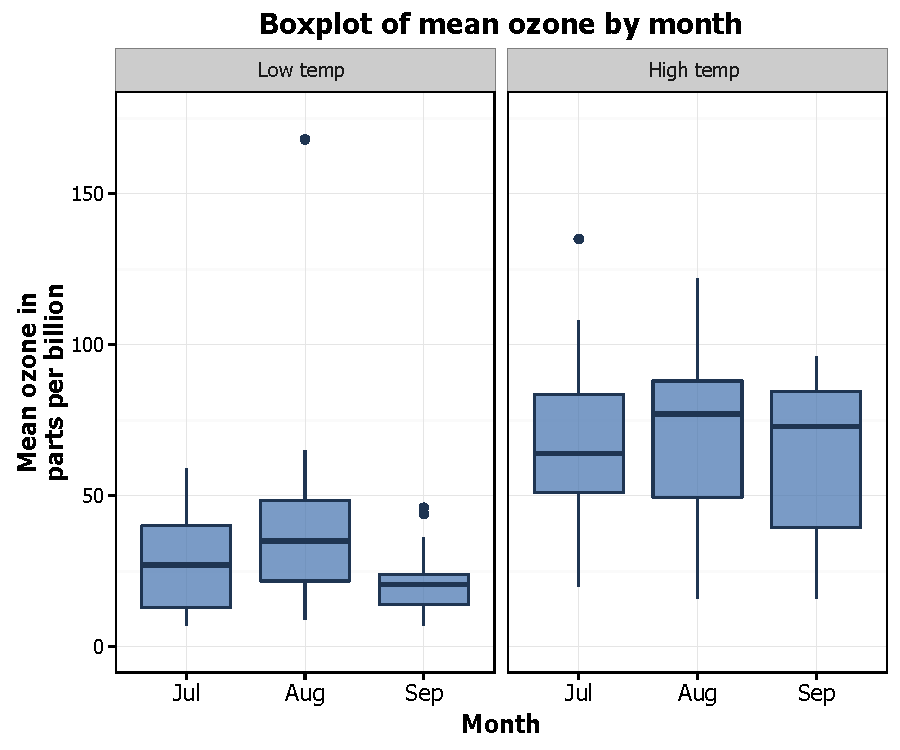
\includegraphics[width=0.6\linewidth]{10_Boxplots_pdf/box_17-1} \end{center}

In order to plot the two Temperature levels in the same plot, we need to
add a couple of things. Firstly, in the \texttt{ggplot} function, we add
a \texttt{fill\ =\ Temp.f} argument to \texttt{aes}. Secondly, we
customise the colours of the boxes by adding the
\texttt{scale\_fill\_brewer} to the plot from the \texttt{RColorBrewer}
package.
\href{http://moderndata.plot.ly/create-colorful-graphs-in-r-with-rcolorbrewer-and-plotly/}{This}
blog post describes the available packages.

\begin{Shaded}
\begin{Highlighting}[]
\NormalTok{p10 <-}\StringTok{ }\KeywordTok{ggplot}\NormalTok{(airquality_trimmed, }\KeywordTok{aes}\NormalTok{(}\DataTypeTok{x =} \NormalTok{Month, }\DataTypeTok{y =} \NormalTok{Ozone, }\DataTypeTok{fill =} \NormalTok{Temp.f)) +}\StringTok{ }
\StringTok{  }\KeywordTok{geom_boxplot}\NormalTok{(}\DataTypeTok{alpha=}\FloatTok{0.7}\NormalTok{) +}
\StringTok{  }\KeywordTok{scale_y_continuous}\NormalTok{(}\DataTypeTok{name =} \StringTok{"Mean ozone in}\CharTok{\textbackslash{}n}\StringTok{parts per billion"}\NormalTok{,}
    \DataTypeTok{breaks =} \KeywordTok{seq}\NormalTok{(}\DecValTok{0}\NormalTok{, }\DecValTok{175}\NormalTok{, }\DecValTok{25}\NormalTok{), }\DataTypeTok{limits=}\KeywordTok{c}\NormalTok{(}\DecValTok{0}\NormalTok{, }\DecValTok{175}\NormalTok{)) +}
\StringTok{  }\KeywordTok{scale_x_discrete}\NormalTok{(}\DataTypeTok{name =} \StringTok{"Month"}\NormalTok{) +}
\StringTok{  }\KeywordTok{ggtitle}\NormalTok{(}\StringTok{"Boxplot of mean ozone by month"}\NormalTok{) +}
\StringTok{  }\KeywordTok{theme_bw}\NormalTok{() +}
\StringTok{  }\KeywordTok{theme}\NormalTok{(}\DataTypeTok{plot.title =} \KeywordTok{element_text}\NormalTok{(}\DataTypeTok{size =} \DecValTok{14}\NormalTok{, }\DataTypeTok{family =} \StringTok{"Tahoma"}\NormalTok{, }\DataTypeTok{face =} \StringTok{"bold"}\NormalTok{),}
    \DataTypeTok{panel.border =} \KeywordTok{element_rect}\NormalTok{(}\DataTypeTok{colour =} \StringTok{"black"}\NormalTok{, }\DataTypeTok{fill=}\OtherTok{NA}\NormalTok{, }\DataTypeTok{size=}\NormalTok{.}\DecValTok{5}\NormalTok{),}
    \DataTypeTok{text =} \KeywordTok{element_text}\NormalTok{(}\DataTypeTok{size =} \DecValTok{12}\NormalTok{, }\DataTypeTok{family =} \StringTok{"Tahoma"}\NormalTok{),}
    \DataTypeTok{axis.title =} \KeywordTok{element_text}\NormalTok{(}\DataTypeTok{face=}\StringTok{"bold"}\NormalTok{),}
    \DataTypeTok{axis.text.x=}\KeywordTok{element_text}\NormalTok{(}\DataTypeTok{size =} \DecValTok{11}\NormalTok{)) +}
\StringTok{  }\KeywordTok{scale_fill_brewer}\NormalTok{(}\DataTypeTok{palette =} \StringTok{"Accent"}\NormalTok{)}
\NormalTok{p10}
\end{Highlighting}
\end{Shaded}

\begin{center}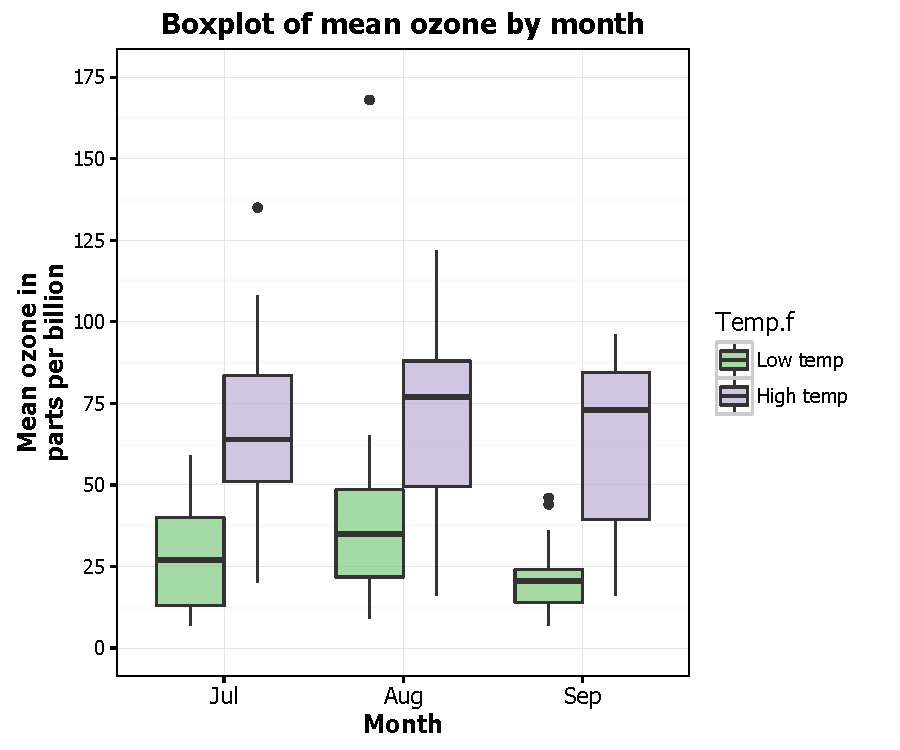
\includegraphics[width=0.6\linewidth]{10_Boxplots_pdf/box_18-1} \end{center}

\section{Formatting the legend}\label{formatting-the-legend}

Finally, we can format the legend. Firstly, we can change the position
by adding the \texttt{legend.position\ =\ "bottom"} argument to the
\texttt{theme} option, which moves the legend under the plot. Secondly,
we can fix the title by adding the
\texttt{labs(fill\ =\ "Temperature\ ")} option to the plot.

\begin{Shaded}
\begin{Highlighting}[]
\NormalTok{p10 <-}\StringTok{ }\KeywordTok{ggplot}\NormalTok{(airquality_trimmed, }\KeywordTok{aes}\NormalTok{(}\DataTypeTok{x =} \NormalTok{Month, }\DataTypeTok{y =} \NormalTok{Ozone, }\DataTypeTok{fill =} \NormalTok{Temp.f)) +}\StringTok{ }
\StringTok{  }\KeywordTok{geom_boxplot}\NormalTok{(}\DataTypeTok{alpha=}\FloatTok{0.7}\NormalTok{) +}
\StringTok{  }\KeywordTok{scale_y_continuous}\NormalTok{(}\DataTypeTok{name =} \StringTok{"Mean ozone in}\CharTok{\textbackslash{}n}\StringTok{parts per billion"}\NormalTok{,}
    \DataTypeTok{breaks =} \KeywordTok{seq}\NormalTok{(}\DecValTok{0}\NormalTok{, }\DecValTok{175}\NormalTok{, }\DecValTok{25}\NormalTok{), }\DataTypeTok{limits=}\KeywordTok{c}\NormalTok{(}\DecValTok{0}\NormalTok{, }\DecValTok{175}\NormalTok{)) +}
\StringTok{  }\KeywordTok{scale_x_discrete}\NormalTok{(}\DataTypeTok{name =} \StringTok{"Month"}\NormalTok{) +}
\StringTok{  }\KeywordTok{ggtitle}\NormalTok{(}\StringTok{"Boxplot of mean ozone by month"}\NormalTok{) +}
\StringTok{  }\KeywordTok{theme_bw}\NormalTok{() +}
\StringTok{  }\KeywordTok{theme}\NormalTok{(}\DataTypeTok{plot.title =} \KeywordTok{element_text}\NormalTok{(}\DataTypeTok{size =} \DecValTok{14}\NormalTok{, }\DataTypeTok{family =} \StringTok{"Tahoma"}\NormalTok{, }\DataTypeTok{face =} \StringTok{"bold"}\NormalTok{), }
    \DataTypeTok{panel.border =} \KeywordTok{element_rect}\NormalTok{(}\DataTypeTok{colour =} \StringTok{"black"}\NormalTok{, }\DataTypeTok{fill=}\OtherTok{NA}\NormalTok{, }\DataTypeTok{size=}\NormalTok{.}\DecValTok{5}\NormalTok{),}
    \DataTypeTok{text =} \KeywordTok{element_text}\NormalTok{(}\DataTypeTok{size =} \DecValTok{12}\NormalTok{, }\DataTypeTok{family =} \StringTok{"Tahoma"}\NormalTok{),}
    \DataTypeTok{axis.title =} \KeywordTok{element_text}\NormalTok{(}\DataTypeTok{face=}\StringTok{"bold"}\NormalTok{),}
    \DataTypeTok{axis.text.x=}\KeywordTok{element_text}\NormalTok{(}\DataTypeTok{size =} \DecValTok{11}\NormalTok{),}
    \DataTypeTok{legend.position =} \StringTok{"bottom"}\NormalTok{) +}
\StringTok{  }\KeywordTok{scale_fill_brewer}\NormalTok{(}\DataTypeTok{palette =} \StringTok{"Accent"}\NormalTok{) +}
\StringTok{  }\KeywordTok{labs}\NormalTok{(}\DataTypeTok{fill =} \StringTok{"Temperature "}\NormalTok{)}
\NormalTok{p10}
\end{Highlighting}
\end{Shaded}

\begin{center}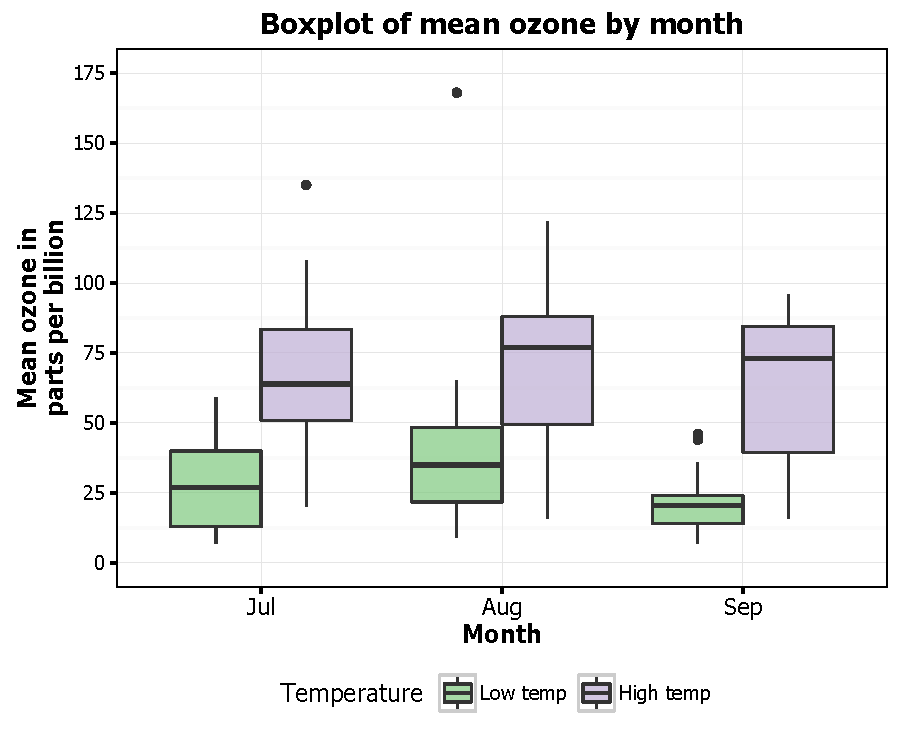
\includegraphics[width=0.6\linewidth]{10_Boxplots_pdf/box_19-1} \end{center}
